% retazosfisica.tex
% Fichero principal
%
% Copyright (C) 2020-2025 José A. Navarro Ramón <janr.devel@gmail.com>
% 1) Código fuente:
% Licencia GNU-2
%
% 2) Texto legible en cualquier formato: pdf, postscript, html, etc.:
% Licencia Creative Commons Recognition-NonCommercial-ShareAlike.
% (CC-BY-NC-SA)
% ----------------------------------------------------------------------------
\documentclass[a4paper,twoside]{book}

% Paquetes
\usepackage{retazosfisica.pkg}

% Definiciones
\usepackage{retazosfisica.defs}

\begin{document}
% -----------------------------------------------------------------------------
% Portada
\thispagestyle{empty}
% portada.tex
% Portada del libro
%
% Copyright (C) 2020-2025 José A. Navarro Ramón <janr.devel@gmail.com>
% 1) Código fuente:
% Licencia GNU-2
%
% 2) Texto legible en cualquier formato: pdf, postscript, html, etc.:
% Licencia Creative Commons Recognition-NonCommercial-ShareAlike.
% (CC-BY-NC-SA)
% ----------------------------------------------------------------------------

% PORTADA
\newcommand*{\titleTH}{\begingroup% T&H Typography
\raggedleft
\vspace*{\baselineskip}
%{\bfseries Apuntes de}\\[\baselineskip]
{\textcolor{red}{\Huge RETAZOS DE FÍSICA\dots}}\\[\baselineskip]
{\large\dots un revuelto de física\dots}\par
\vspace{2ex}
{\large\today}\par
\vspace{10ex}
{\Large José A. Navarro Ramón}\\[0.167\textheight]
\vspace{20ex}
{\Large 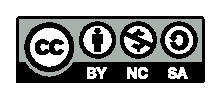
\includegraphics[width=3.0cm]{./img/static/Cc-by-nc-sa_icon.eps}}\par
\vspace*{3\baselineskip}
\endgroup}

\titleTH


%%% Local Variables:
%%% mode: latex
%%% TeX-engine: luatex
%%% TeX-master: "../retazosfisica.tex"
%%% End:



% -----------------------------------------------------------------------------
% Tabla de contenidos
\thispagestyle{empty}
% tablacontenidos.tex
% Tabla de contenidos.
%
% Copyright (C) 2020-2025 José A. Navarro Ramón <janr.devel@gmail.com>
% 1) Código fuente:
% Licencia GNU-2
%
% 2) Texto legible en cualquier formato: pdf, postscript, html, etc.:
% Licencia Creative Commons Recognition-NonCommercial-ShareAlike.
% (CC-BY-NC-SA)
% ----------------------------------------------------------------------------

\tableofcontents

%%% Local Variables:
%%% mode: latex
%%% TeX-engine: luatex
%%% TeX-master: ../mcfeynman.tex
%%% End:

% -----------------------------------------------------------------------------
\frontmatter
% prologo.tex
%
% Copyright (C) 2025 José A. Navarro Ramón <janr.devel@gmail.com>
% Licencia Creative Commons Recognition Share-alike.
% (CC-BY-SA)

\chapter{Prólogo}



 
%%% Local Variables:
%%% mode: latex
%%% TeX-engine: luatex
%%% TeX-master: "../retazosfisica.tex"
%%% End:

% -----------------------------------------------------------------------------
% Teoría
\mainmatter
%\part{Teoría}
% mecanicaestadistica.tex
%
% Copyright (C) 2025 José A. Navarro Ramón <janr.devel@gmail.com>
% Licencia Creative Commons Recognition Share-alike.
% (CC-BY-SA)

\chapter{Mecánica estadística}
La mecánica estadística es una herramienta muy útil en física para estudiar
las propiedades macroscópicas de un sistema que está formado por un número
enrome de partículas, sin tener en cuenta el estado de todas y cada una de
ellas. Esto se lleva a cabo encontrando la configuración más probable de
las partículas.

Este capítulo se desarrolla a nivel básico la mecánica estadística
de Maxwell-Boltzmann, la de Bose-Einstein y la de Planck.

\section{Estadística de Maxwell-Boltzmann}
Boltzmann fue un físico austriaco pionero de la mecánica estadística y se
encontró con la incomprensión de muchos físicos de su tiempo, pues el
atomismo no estaba del todo aceptado. Al poco de morir ---comienzos del siglo
XX--- se acumularon más evidencias a favor de los átomos, de modo que esta
quedó completamente aceptada poco después.
%[Wikipedia]

\subsection{Modelo teórico}
En este modelo, se considera un sistema aislado formado por un número enorme
$N$ de partículas distinguibles de cualquier spin y que están lo
suficientemente separadas entre sí como para que la única interacción entre
ellas sea una colisión elástica; por tanto, se desprecia la interacción a
distancia, esto es, la energía potencial de cualquier tipo.
% [Arthur Beiser]

Un ejemplo típico al que se le puede aplicar el modelo es el de un gas formado
por moléculas ---átomos o grupos de átomos neutros---.

Las $N$ partículas, $n_1, n_2, \cdots, n_k$, se distribuyen entre $k$ estados
de energía creciente,  $u_1, u_2, \cdots, u_k$ . Estos estados pueden ser,
bien estados discretos o energías medias de una secuencia creciente de
intervalos continuos. Incluso, como el modelo es clásico, el número de niveles
$k$ puede ser muy elevado, y se podría considerar que estas forman un
continuo (esto lo utilizaremos más tarde).

En todo momento se conserva el número de partículas y la energía.
\begin{equation}
  \sum_{i=1}^{k} n_i = N
\end{equation}
y la energía:
\begin{equation}
  \sum_{i=1}^{k} n_i u_i = U
\end{equation}












%%% Local Variables:
%%% mode: latex
%%% TeX-engine: luatex
%%% TeX-master: "../retazosfisica.tex"
%%% End:

% matrizdensidad.tex
%
% Copyright (C) 2020-2025 José A. Navarro Ramón <janr.devel@gmail.com>
% 1) Código fuente:
% Licencia GNU-2
%
% 2) Texto legible en cualquier formato: pdf, postscript, html, etc.:
% Licencia Creative Commons Recognition-NonCommercial-ShareAlike.
% (CC-BY-NC-SA)
% ----------------------------------------------------------------------------

\chapter{Matriz Densidad}

\section{Introducción}
Vamos a utilizar un espacio de Hilbert $\left(\mathbb{C}^2\right)$, de
dimensión 2, por comodidad
\[
  \mathlarger{\mathcal{H} = \mathbb{C}^2}
\]

Lo siguiente es elegir los símbolos de una base. Se podrían elegir algunos
símbolos como $\ket{\varphi_1}$ y $\ket{\varphi_2}$, $\ket{e_1}$ y $\ket{e_2}$,
$\ket{a}$ y $\ket{b}$, etc. Pero vamos a introducir una nomenclatura que es
propia de la información cuántica y que hace referencia al \emph{qbit}.
De esta forma, la base\footnotemark{} la representaríamos como
\footnotetext{La base está formada por dos vectores en un espacio de Hilbert
  de dimensión 2. En general, tendría $n$ vectores.}
\[
  B = \{\ket{0}, \ket{1}\}
\]

El cero y el uno son solo etiquetas. No hay nada profundo en eso, solo inspiran
al bit clásico. Únicamente decir, por completitud, que por \emph{qbit} se
entiende aquel vector que es una combinación lineal de estos dos vectores de la
base
\[
  \ket{\Psi} = a \ket{0} + b \ket{1}
\]
pero no vamos a entrar en esto. Dejamos los \emph{qbits} a un lado.

A partir de ahora solo consideramos tener un espacio de Hilbert de dimensión 2
y estos dos vectores de la base.

Como es costumbre cuando se trabaja en un espacio de dimensión finita, podemos
utilizar una expresión matricial. Así, podremos representar los vectores de la
base como
\[
  \ket{0} = \begin{pmatrix}1 \\ 0\end{pmatrix}
  \hspace{4em}
  \ket{1} = \begin{pmatrix}0 \\ 1\end{pmatrix}
\]
y sus duales
\[
  \bra{0} = \ket{0}^\dagger
  = \begin{pmatrix}1 \\ 0\end{pmatrix}^\dagger
  = \begin{pmatrix}1 & 0\end{pmatrix}
  \hspace{4em}
  \bra{1} = \ket{1}^\dagger
  = \begin{pmatrix}0 \\ 1\end{pmatrix}^\dagger
  = \begin{pmatrix}0 & 1\end{pmatrix}
\]

\subsection{Operadores autoadjuntos}
En mecánica cuántica, un operador está asociado a un observable si el adjunto
del operador coincide con él mismo, de manera que sus valores propios serían
reales. Un operador así se llama autoadjunto
\[
  \hat{A}^\dagger = \hat{A}
\]

Cuando un operador $\hat{A}$ es autoadjunto, se puede encontrar una nueva base
propia del operador
\[
  \{\ket{a_1}, \ket{a_2}\}
\]
que, por ser base es ortogonal, y por ser autoadjunto, sus valores propios son
reales
\begin{align*}
  &\hat{A} \ket{a_1} = \lambda_1 \ket{a_1}\\
  &\hat{A} \ket{a_2} = \lambda_2 \ket{a_2}
\end{align*}
donde $\lambda_{1}, \lambda_{2} \in \mathbb{R}$.
Recordemos que estamos en un espacio de dimensión 2, pero esto también es
válido para un espacio finito de dimensión superior.
A menos que se diga lo contrario, los operadores que nos encontremos serán
autoadjuntos.

\subsection{Valor esperado de un operador}
Supongamos que un sistema está descrito por el estado $\ket{\Psi}$. Nos
preguntamos acerca del valor esperado de un operador cuando el sistema está en
ese estado.

Si estamos en un mundo de dimensión 2, y la base que utilizamos es
$\{\ket{0}, \ket{1}\}$, el estado se puede expresar como una combinación lineal
de los vectores de la base
\[
  \ket{\Psi} = a_0 \ket{0} + a_1 \ket{1}
  \text{, donde }
  a_i \in \mathbb{C}
\]

Se define el \emph{valor esperado del observable} $\hat{A}$, cuando el sistema
está en el estado $\ket{\Psi}$, mediante el producto escalar
\begin{align*}
  \braket{\hat{A}}_{\Psi}
  &= \braket{\Psi | \hat{A} | \Psi}
  = \left(a_{0}^{*} \bra{0} + a_{1}^{*} \bra{1}\right)
  \hat{A}
    \left(a_{0} \ket{0} + a_{1} \ket{1}\right)\\
  &= a_{0}^{*} a_{0} \braket{0|\hat{A}|0}
    + a_{0}^{*} a_{1} \braket{0|\hat{A}|1}
    + a_{1}^{*} a_{0} \braket{1|\hat{A}|0}
    + a_{1}^{*} a_{1} \braket{1|\hat{A}|1}\\
  &= a_{0} a_{0}^{*} \braket{0|\hat{A}|0}
    + a_{1} a_{0}^{*} \braket{0|\hat{A}|1}
    + a_{0} a_{1}^{*} \braket{1|\hat{A}|0}
    + a_{1} a_{1}^{*} \braket{1|\hat{A}|1}\\
  &= a_{0} a_{0}^{*} A_{00}
    + a_{1} a_{0}^{*} A_{01}
    + a_{0} a_{1}^{*} A_{10}
    + a_{1} a_{1}^{*} A_{11}\\
  &= \rho_{00} A_{00}
    + \rho_{10} A_{01}
    + \rho_{01} A_{10}
    + \rho_{11} A_{11}
\end{align*}
donde hemos utilizado $A_{ij} = \braket{i|\hat{A}|j}$.

Si ahora llamamos $\rho_{ij} = a_{i} a_{j}^{*}$, obtenemos
\begin{equation}
  \braket{\hat{A}}_{\Psi}
  = \braket{\Psi | \hat{A} | \Psi}
  = \rho_{00} A_{00}
    + \rho_{10} A_{01}
    + \rho_{01} A_{10}
    + \rho_{11} A_{11}  
\end{equation}
Obsérvese que el valor esperado de un operador autoadjunto es un número real.

Las $\rho_{ij}$ las podríamos interpretar como elementos de una matriz $2\times 2$.
Por otro lado, sabemos por mecánica cuántica que las $A_{ij}$ son elemenntos de una
matriz. Así que
\[
  \mmm{\rho}
  = \begin{pmatrix}\rho_{00} & \rho_{01} \\ \rho_{10} & \rho_{11} \end{pmatrix}
  ;\hspace{4em}
  \mmm{A}
  = \begin{pmatrix}A_{00} & A_{01} \\ A_{10} & A_{11} \end{pmatrix}
\]

Pero, al multiplicar estas dos matrices $2\times 2$ obtenemos otra matriz
$2\times 2$, no un número, aunque, si nos fijamos en los elementos diagonales
\[
  \mmm{\rho} \mmm{A}
  = \begin{pmatrix}\rho_{00} & \rho_{01} \\ \rho_{10} & \rho_{11} \end{pmatrix}
  \begin{pmatrix}A_{00} & A_{01} \\ A_{10} & A_{11} \end{pmatrix}
  = \begin{pmatrix}
    \rho_{00} A_{00} + \rho_{01} A_{10} & \cdots \\
    \cdots & \rho_{10} A_{01} + \rho_{11} A_{11}
  \end{pmatrix}
\]

Pero, si nos fijamos en los elementos diagonales, observamos que el valor
esperado es la suma de estos. La suma de los elementos diagonales de una matriz
cuadrada es la \emph{traza}
\[
  \braket{\hat{A}}_{\Psi}
  = \braket{\Psi|\hat{A}|\Psi}
  = \text{Tr}(\mmm{\rho}\mmm{A})
\]

¿Por qué nos complicamos tanto para calcular el valor esperado de un observable
en el estado $\ket{\Psi}$, si lo podemos calcular directamente como
$\braket{\Psi|\hat{A}|\Psi}$?

Bueno, sí y no. Resulta que en estadística, o incluso, en teoría de información
cuántica, puede ocurrir que nos digan que la probabilidad de que un sistema se
encuentre en un estado, digamos, $\ket{\alpha}$, sea $1/3$ y que la de
encontrarse en $\ket{\beta}$ fuera $2/3$. Es decir, que no nos aseguren que el
sistema se encuentre en un estado cuántico concreto.

Este tipo de situación introduce una incertidumbre clásica, pues estas
probabilidades son absolutamente clásicas. Además, en los estados cuánticos
$\ket{\alpha}$ y $\ket{\beta}$ también hay probabilidades cuánticas.

Todo esto nos complica bastante la vida, y su desarrollo sería muy laborioso,
muy difuso y muy poco claro, si utilizamos la nomenclatura estándar del cálculo
vectorial de toda la vida, y resulta que introduciendo esta matriz densidad
$\mmm{\rho}$, todo es mucho más fácil e intuitivo.

Podemos observar que la matriz densidad depende solo de los coeficientes de la
función de onda en nuestra base, $\ket{\Psi} = a_0 \ket{0} + a_1 \ket{1}$
\[
  \mmm{\rho]}
  = \begin{pmatrix}\rho_{00} & \rho_{01}\\ \rho_{10} & \rho_{11}\end{pmatrix}
  = \begin{pmatrix}
    a_{0} a_{0}^{*} & a_{0} a_{1}^{*} \\
    a_{1} a_{0}^{*} & a_{1} a_{1}^{*}
    \end{pmatrix}
\]


\subsection{Estado puro}
Ahora mostraremos otra forma de obtener la matriz densidad
\[
  \ket{\Psi}\bra{\Psi}
  = \begin{pmatrix}a_0 \\ a_1\end{pmatrix}
  = \begin{pmatrix}a_{0}^{*} & a_{1}^{*}\end{pmatrix}
  = \begin{pmatrix}
    a_{0} a_{0}^{*} & a_{0} a_{1}^{*} \\
    a_{1} a_{0}^{*} & a_{1} a_{1}^{*}
  \end{pmatrix}
  = \mmm{\rho}
\]

Decimos que un sistema se encuentra en un estado cuántico puro si
\begin{equation}
  \mmm{\rho} = \ket{\Psi} \bra{\Psi}
\end{equation}

\section{Propiedades de la matriz densidad}
\begin{enumerate}
\item {\bfseries $\mmm{\rho}$ es un Operador autoadjunto.}
  Un operador $\mmm{\hat{A}}$ es autoadjunto si
  $\mmm{\hat{A}}^\dagger = \mmm{\hat{A}}$
  \begin{align*}
    \mmm{\rho}^\dagger
    &= \begin{pmatrix}
      a_0 a_0^* & a_0 a_1^* \\
      a_1 a_0^* & a_1 a_1^*
    \end{pmatrix}^\dagger
    = \begin{pmatrix}
      (a_0 a_0^*)^* & (a_1 a_0^*)^* \\
      (a_0 a_1^*)^* & (a_1 a_1^*)^*
    \end{pmatrix}\\
    &= \begin{pmatrix}
      a_0^* a_0 & a_1^* a_0 \\
      a_0^* a_1 & a_1^* a_1
    \end{pmatrix}
    = \begin{pmatrix}
      a_0 a_0^* & a_0 a_1^* \\
      a_1 a_0^* & a_1 a_1^*
    \end{pmatrix}
    = \mmm{\rho}
  \end{align*}

  Por tanto, la matriz densidad representa a un operador autoadjunto.
  A partir de ahora representaremos de manera apropiada a este operador,
  con el acento circunflejo, $\mmm{\hat{\rho}}$. Este operador describe el
  estado de un sistema cuántico.
  
\item {\bfseries La traza de la matriz densidad es la unidad.}
  La traza de una matriz cuadrada es la suma de sus elementos diagonales.
  \[
    \mmm{\hat{\rho}}
    = \begin{pmatrix}
      a_0 a_0^* & a_0 a_1^* \\
      a_1 a_0^* & a_1 a_1^*
    \end{pmatrix}
  \]

  \[
    \text{Tr}(\mmm{\hat\rho})
    = a_0 a_0^* + a_1 a_1^*
    = |a_0|^2 + |a_1|^2 = 1
  \]

  Como $a_0$ y $a_1$ son las componentes del vector de estado del sistema, que
  está normalizado, la suma de los cuadrados de sus módulos debe valer la
  unidad.
  \[
    \ket{\Psi} = a_0 \ket{0} + a_1 \ket{1}
  \]

\item {\bfseries El operador $\mmm{\hat{\rho}}$ es positivo
    ($\mmm{\hat{\rho}} > 0$).}
  Esto quiere decir que para cualquier ket $\ket{u}$ en nuestro espacio de
  Hilbert, se debe cumplir
  \[
    \braket{u|\mmm{\hat{\rho}}|u} > 0
  \]

  Otra manera de decirlo es que, dado que $\mmm{\hat{\rho}}$ es autoadjunto, se
  puede diagonalizar (expresarse en su base propia) y los valores propios, aquí
  $\lambda_1$ y $\lambda_2$, deben ser no negativos
  \[
    \mmm{\hat{\rho}}
    = \begin{pmatrix}\lambda_1 & 0 \\ 0 \lambda_2\end{pmatrix}
    \hspace{2em}\text{con } \lambda_1, \lambda_2 \geq 0    
  \]
  
  Obsérvese que, aunque los valores propios han de ser no negativos, no pueden
  ser ambos cero, pues la traza de la matriz debe valer la unidad.
\end{enumerate}

Como resumen, recordamos que para que una matriz $\mmm{\hat{\rho}}$ pueda ser
considerada matriz densidad, debe tener las tres propiedades que presentamos de
forma simbólica
\begin{enumerate}
\item $\mmm{\hat{\rho}}^\dagger = \mmm{\hat{\rho}}$
\item $\text{Tr}(\mmm{\hat\rho}) = 1$
\item $\mmm{\hat{\rho}} > 0$
\end{enumerate}

\subsection{Combinación lineal de matrices densidad}
Ahora nos interesa saber si una combinación lineal de matrices densidad, como
\[
  \mmm{\hat{\rho}} = \alpha \mmm{\hat{\rho}}_1 + \beta \mmm{\hat{\rho}}_2
\]
es también una matriz densidad.

Para que esto sea así, la combinación lineal debe cumplir las tres propiedades
anteriores.

Fijémonos en la tercera propiedad ($\mmm{\hat{\rho}}$, como
$\mmm{\hat{\rho}}_1$ y $\mmm{\hat{\rho}}_2$ son matrices densidad, ambas son
positivas, $\mmm{\hat{\rho}}_1 > 0$ y $\mmm{\hat{\rho}}_2 > 0$. Podremos decir,
sin demostrar, que si los coeficientes $\alpha$ y $\beta$ son números reales
positivos
\[
  \alpha, \beta \in \mathbb{R}^{+} \cup \set{0}
\]
entonces la combinación lineal sería definida positiva.

También podríamos demostrar que si $\mmm{\hat{\rho}}_1$ y $\mmm{\hat{\rho}}_2$
son operadores autoadjuntos y $\alpha$ y $\beta$ son números reales, entonces,
$\mmm{\hat{\rho}}$ también es autoadjunta.

Nos queda el valor de la traza de la combinación lineal. La traza es una
operación lineal, y por tanto
\[
  \text{Tr}{\mmm{\hat\rho}}
  = \text{Tr}(\alpha \mmm{\hat{\rho}}_1 + \beta \mmm{\hat{\rho}}_2)
  = \alpha\,\text{Tr}(\mmm{\hat{\rho}}_1)+\beta\,\text{Tr}(\mmm{\hat{\rho}}_2)
    = \alpha \cdot 1 + \beta \cdot 1
    = \alpha + \beta
\]
Luego, para que se cumpla $\text{Tr}\mmm{\hat{\rho}} = 1$, la suma de los
coeficientes debe valer la unidad
\[
  \alpha + \beta = 1
\]

Hemos llegado a la conclusión de que si construyo una nueva matriz densidad
mediante una combinación lineal de otras, obtendré una matriz densidad, con
tal de que los coeficientes sean reales no negativos y sumen la unidad.
\[
  \mmm{\hat{\rho}} = \sum_i P_i \mmm{\hat{\rho}}_i
  \text{, con } P_i \geq 0 \text{ y } \sum_i P_i = 1
\]

Esta propiedad tiene que ver con una distribución de probabilidad discreta
clásica.






%%% Local Variables:
%%% mode: latex
%%% TeX-engine: luatex
%%% TeX-master: "../retazosfisica.tex"
%%% End:

% -----------------------------------------------------------------------------
%% Apéndices
%%\backmatter
%%\part{Apéndices}
%\appendix
%\renewcommand{\thechapter}{A}
%\clearpage
%\addappheadtotoc
%\appendixpage
%%\include{./apendices/gl-momangcuantico-genfunciones}
% -----------------------------------------------------------------------------

\end{document}


%%% Local Variables:
%%% coding: utf-8
%%% mode: latex
%%% TeX-engine: luatex
%%% TeX-master: t
%%% End:
